\chapter{Introduction}

An overarching goal in human genetics is to understand the relationship between genotype and phenotype. An integral step is toward this goal is learning how to interpret the functional consequences of genetic variants. In protein-coding regions, it is relatively easy to predict if a single nucleotide polymorphism \emph{(SNP)} will affect protein sequence because the amino acid code is known. However, protein-coding genetic sequence makes up only $\sim1$\% of the genome. Although non-coding regions of the genome were categorized as "junk DNA" for decades, it is now clear that a large proportion of the non-coding genome is essential. Indeed, non-coding DNA has been established to play a large role in gene regulation - the chain of events controlling how and when cells express particular genes. Thus, understanding how non-coding genetic variants influence gene regulation is a vital step toward understanding the relationship between genotype and phenotype. 

In this chapter, I will introduce the two approaches that I have taken in my work to study gene regulation. By providing examples, primarily from the Gilad lab, I will motivate why I have chosen to study gene regulation through quantitative genetics and comparative primate functional genomics. Following this discussion, I argue that co-transcriptional gene regulatory mechanisms remain understudied and warrant particular attention by both approaches. I conclude the chapter with an overview of the remaining chapters in this dissertation.  


\section{Quantitative genetic approaches to understand gene regulation}

Quantitative trait loci \emph{(QTL)} mapping is a tool used to identify genetic variation affecting gene regulation. For example, an expression QTL, or eQTL, is a genetic variant that is statistically associated with mRNA expression.  Over the last decade, a large number of eQTL mapping studies have identified genetic variants with regulatory potential in a wide range of human cell lines and tissues \citep{lappalainen_transcriptome_2013, stranger_population_2007, stranger_population_2007, pickrell_understanding_2010, gtex_consortium_genetic_2017, schmiedel_impact_2018}. In the most comprehensive project to date, the Genome-Tissue Expression \emph{(GTEx)} Consortium generated eQTL maps for over 50 human tissues collected from over 800 healthy individuals \citep{ward_cracking_2017, aguet_gtex_2019, gtex_consortium_genetic_2017}. Integration of these maps has revealed numerous eQTLs for the majority of protein coding genes.  

While eQTLs have been largely successful in identifying SNPs with regulatory potential, this approach does not reveal the chain of events controlling gene expression levels. eQTLs represent a collection of SNPs mediating gene expression along the gene regulatory cascade through a wide range of mechanisms \ref{fig:eQTLMech} \citep{Pai2015}. The development of methods like DNAse-seq \citep{song_dnase-seq_2010} ChIP-Seq \cite{barski_high-resolution_2007}, and ATAC-seq \citep{buenrostro_atac-seq_2015}, which are used to identify chromatin states, made it possible to study the contribution of specific molecular mechanisms to variation in gene expression levels. For example, if we assume an eQTL acts by perturbing a particular mechanism (i.e. chromatin conformation), the SNP should also be associated with measures of that mechanism, and molecular QTL mapping further contributes to the understanding of gene regulation. 


\begin{figure}
\centering
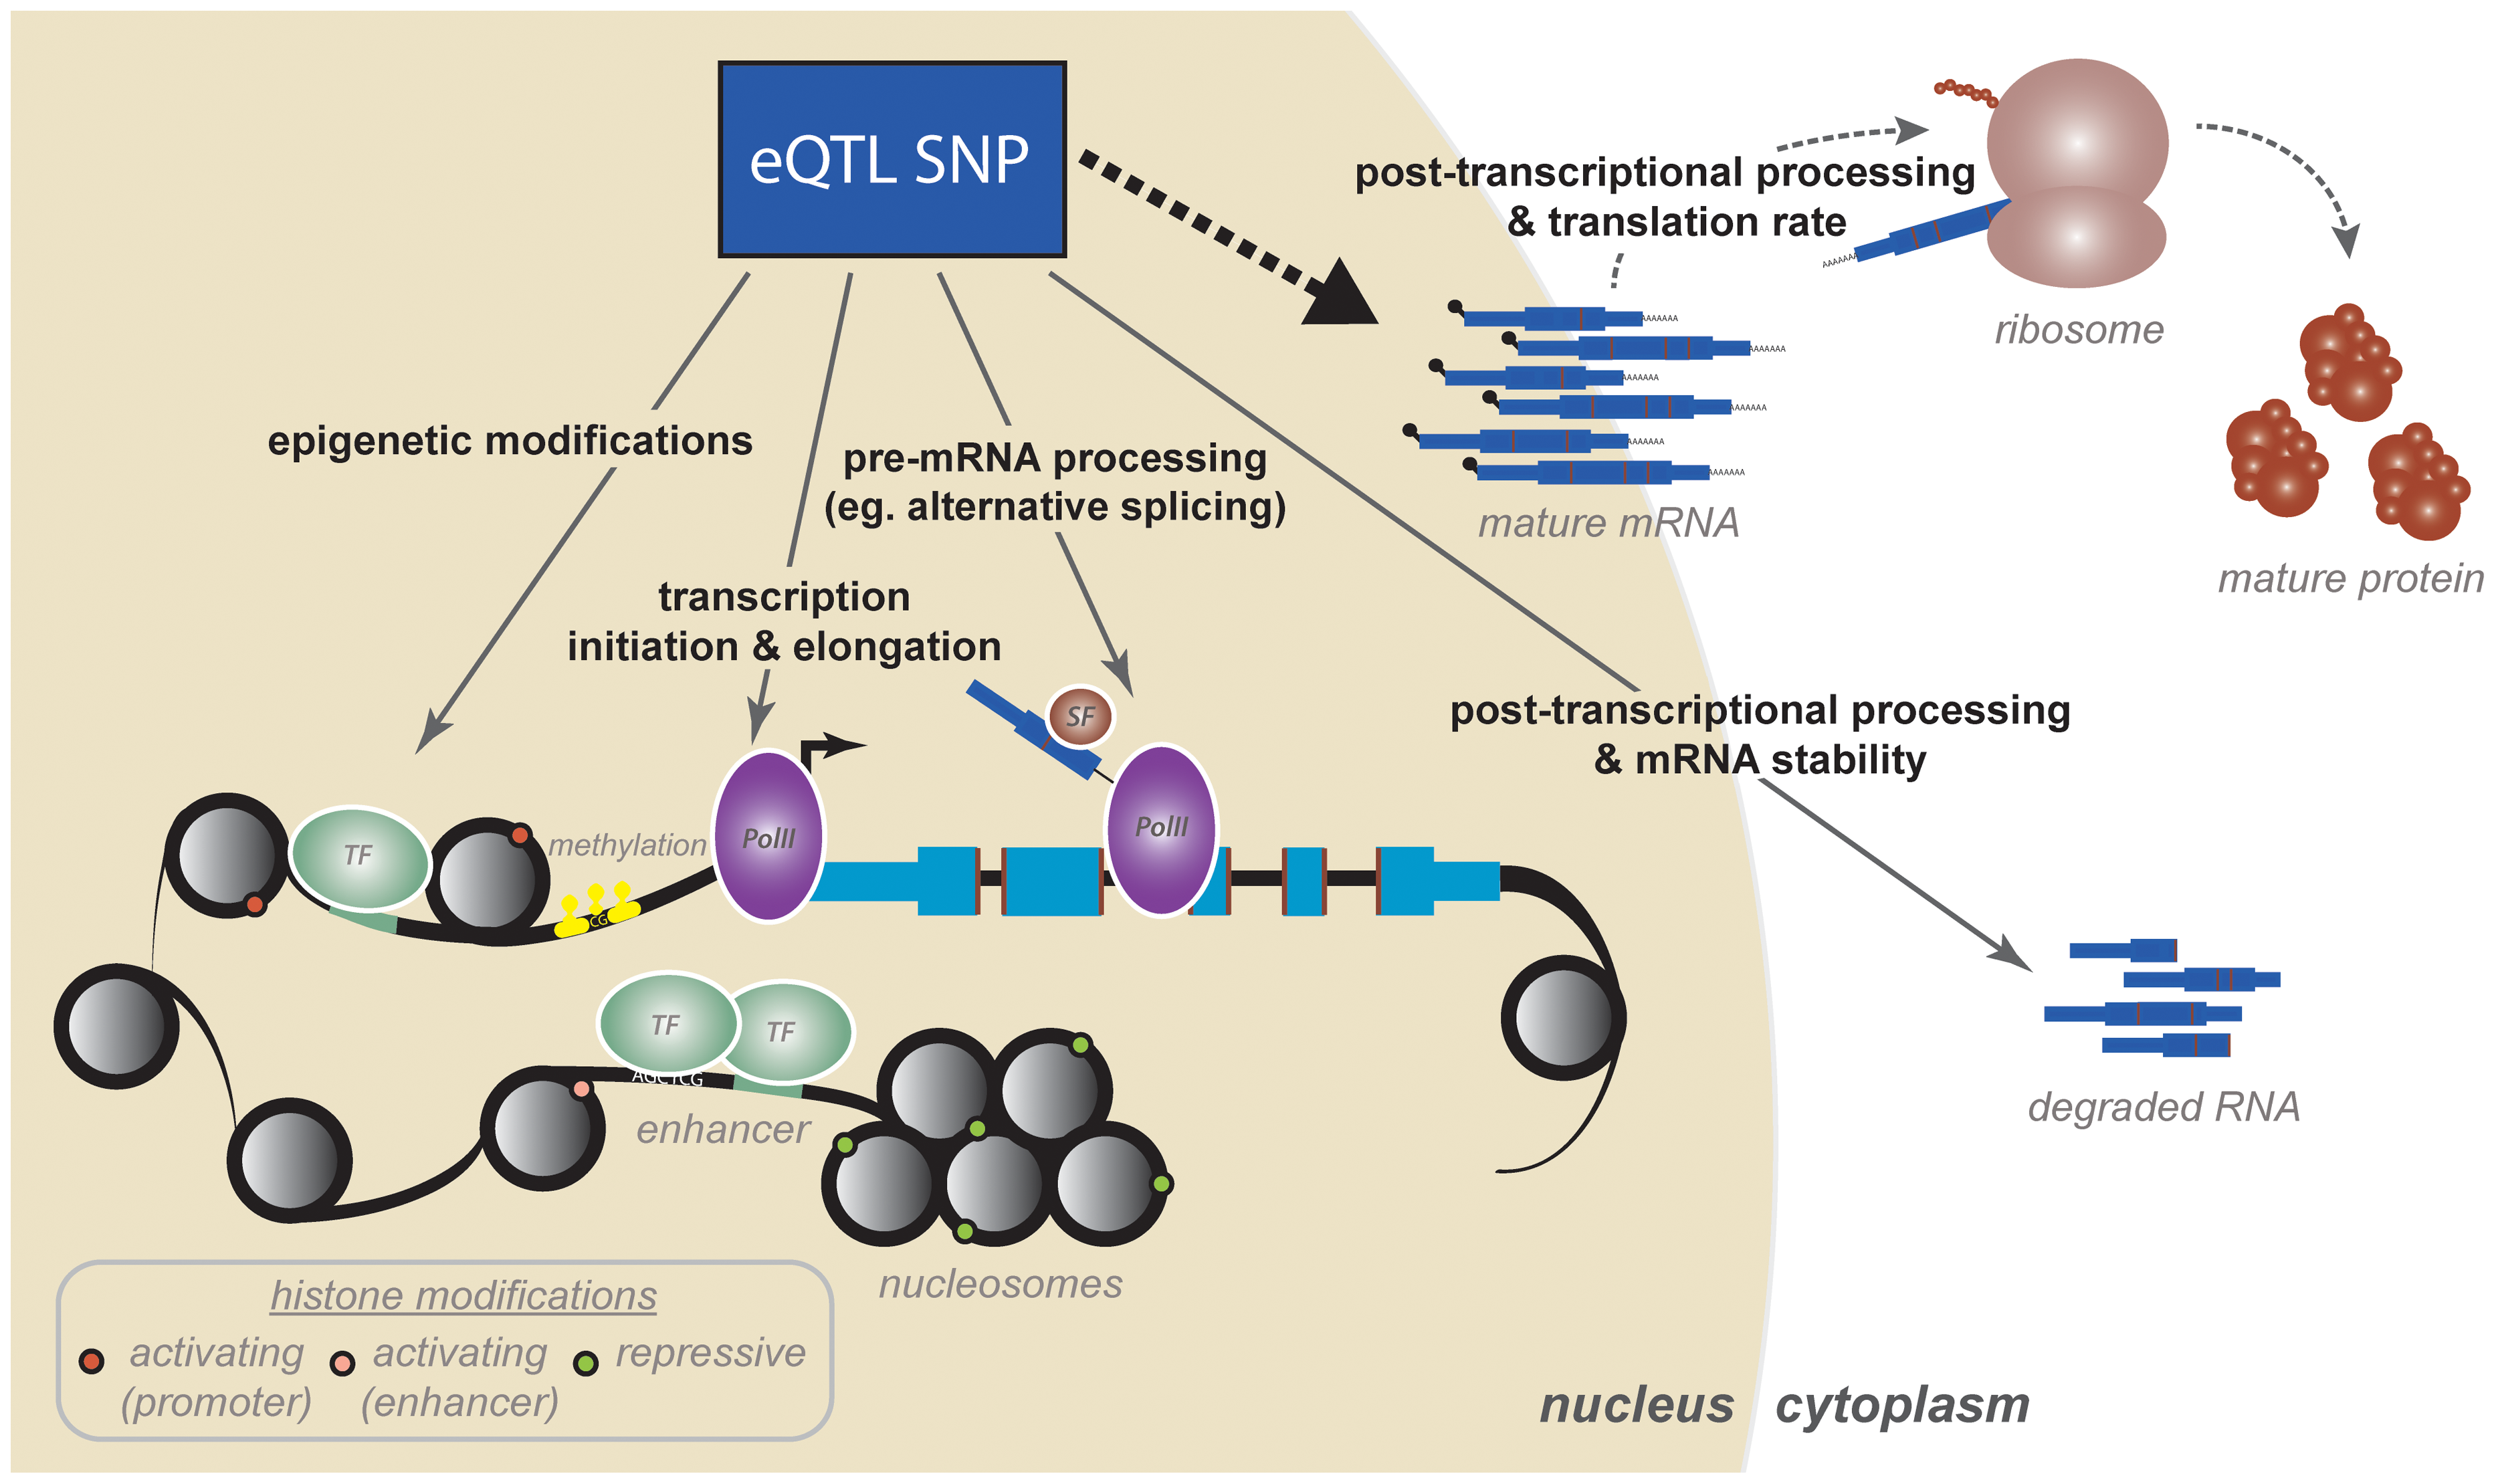
\includegraphics[width=5in]{img/ch01/eQTLMech.png}
\caption[Potential mechanisms for eQTLs]{Figure 1 from Pai, Pritchard, and Gilad 2015 \citep{Pai2015} Regulatory QTL studies have revealed how eQTLs can affect variation in mature mRNA expression levels as well as how variation in mRNA expression may then impact post transcriptional and translational mechanisms.} 
\label{fig:eQTLMech}
\end{figure}

\section{Comparative approaches to understand gene regulation}

Comparative primate functional genomic studies have also contributed to our understanding of human gene regulation. Like phenotypic variation between individual human, phenotypic differences between human and non-human primates stem largely from differences in gene regulation \citep{King1975, carroll_evolution_2005, gilad_expression_2006, wray_evolutionary_2007, blekhman_gene_2008, karaman_comparative_2003}. In turn, primate functional genomic studies complement human-specific quantitative genetic studies. Due to the challenges associated with obtaining primate tissues, comparative studies in primates typically rely on smaller sample sizes. However, these are sufficient to detect the large differences in regulatory mechanisms between species. Comparative genomic approaches also contextualize gene regulatory mechanisms in an evolutionary framework to provide additional insight into which processes or loci are critical to genome and organismal function. 

There are some regulatory processes that, while functionally important, are indistinguishable in human populations or are measured with technology not feasible to use at the scale necessary for quantitative genetic studies. Because genetic variation is larger between species than within human populations, it is possible to distinguish differences in regulatory features between species - even with small sample sizes. For example, before it became technically and financially feasible to measure chromosome contacts genome-wide, Eres \emph{et al.} demonstrated that differences in contact frequencies at individual loci between human and chimpanzee can explain previously identified differentially expressed genes \citep{eres_reorganization_2019}. Specifically, Eres \emph{et al.} used Hi-C to characterize 3D chromatin contacts in human and chimpanzee induced pluripotent stem cells \emph{iPSCs}. At a resolution of 10 kb, they identified 13,572 of the 347,206 ($\sim$4\%) chromatin contacts genome wide to be divergent between species \citep{eres_reorganization_2019}. While a quantitative genetics study to detect significant differences in chromatin interactions between humans was not feasible, this work demonstrated that chromatin contact variation likely mediates differences in gene expression, and complemented previous work that suggested direct contact between distal enhancer elements and promoters driving gene expression \citep{carter_long-range_2002, krivega_enhancer_2012, tolhuis_looping_2002, palstra_-globin_2003, marsman_long_2012}.

Comparative primate genome studies also provide evolutionary context for genetic Comparative primate genome studies also provide evolutionary context for genetic mechanisms and genomic loci previously studied with alternative approaches. Under the assumption that conserved processes and loci are critical to function, understanding evolutionary context of gene regulatory mechanisms can help catalog importance of each mechanism \citep{housman_prime_2020}. For example, human quantitative genetics approaches revealed higher variation in mRNA transcript levels than protein levels, which likely result from mechanisms downstream of translation buffer protein levels \citep{battle_impact_2015}. However, the importance of post-translational gene regulation for maintaining protein level variation was unclear. Wang \emph{et al}, measured translation in a set of primate LCLs with available mRNA expression and protein levels. Using these data, the authors demonstrate that post-translation protein buffering likely plays a large role in shaping primate protein level divergence \citep{wang_posttranslational_2018}. Overall, characterizing gene regulatory mechanisms in both humans and non-human primates is critical to understanding the broader relationship between genotype and phenotype. 

\section{Open questions in how isoform diversity contributes to gene regulation}

Both human population genomic and primate comparative genomic approaches have improved our ability to interpret noncoding variation, yet more work is necessary to understand the gene regulatory code.  It has become clear that a large number of highly conserved genetic variants that correlate with variation in both mRNA expression and complex traits lie in cis-regulatory elements such as promoters and enhancers \citep{maurano_systematic_2012, Trynka2013, zhou_epigenetic_2014}. While considerable effort has been devoted to annotating promoters and enhancers across cell types and species \citep{bernstein_nih_2010, the_encode_project_consortium_integrated_2012, mouse_encode_consortium_encyclopedia_2012, modencode_consortium_unlocking_2009}, a large proportion of variants associated with gene expression variation and/or complex traits remain unannotated and unexplained.

Indeed, the majority of previously explored gene regulatory mechanisms affect gene expression levels pre-transcriptionally through chromatin level variation at promoters and enhancers. However, co-transcriptional mechanisms, such as alternative mRNA splicing and alternative polyadenylation \emph{(APA)}, contribute to both variation in mRNA and protein isoforms dependent on and independent of changes in mRNA expression levels. Understanding the co-transcriptional mechanisms that mediate isoform diversity is a key path forward to predicting phenotype from genotype.  Thus, a greater understanding of how genetic variation and regulatory elements control alternative splicing and APA will fill a gap in predictive models of gene regulation from DNA sequences.

In recent years, a number of groups have started to identify and characterize the genetic variation associated with alternative splicing \emph{(sQTLs)} \citep{takata_genome-wide_2017, li_rna_2016, ongen_alternative_2015, ma_splicing_2018, tian_cancersplicingqtl_2019}. In one such study, Li \emph{et al.} mapped sQTLs in a population of LCLs that was previously used to characterize a number of other molecular QTLs. They reported that most sQTLs, including some previously implicated in GWAS, are not eQTLs \citep{li_rna_2016}. This work suggests genetic variation can mediate traits independently from differences in mRNA expression levels. 

Although comparative functional genomic studies of alternative splicing are still rare, a few studies have generated important insights. Blekhman \emph{et al.} reported that genes with human-specific exon usage are enriched in genes involved in anatomical structure \citep{blekhman_sex-specific_2010}. Additional work has demonstrated how alternative splicing may contribute specifically to differential expression and translation of genes between closely related primates \citep{lin_evolution_2010, attig_splicing_2016}. For example, Attig \emph{et al.} reported that co-evolution of splice sites and U-rich elements in primates has led to an increase in expression of exons containing Alu transposable elements. Their experiments demonstrated inclusion of Alu exons causes down regulation of transcripts through non-sense mediated decay \cite{attig_splicing_2016}.

 Like alternative splicing, cleavage and polyadenylation in introns leads to differential inclusion of coding sequences. mRNA transcripts resulting from intronic polyadenylation are either subject to decay or are translated to distinct protein isoforms (reviewed in Tian and Manley \citep{tian_alternative_2017}). Unlike alternatively spliced transcripts, APA in 3' untranslated regions (3' UTRs) produces transcripts with the same coding sequences thus only differing in 3' UTR length. Variation in downstream regulation of 3' UTR APA isoforms result from differential inclusion of miRNA binding sites and other motifs signaling RNA binding proteins. Thus, isoforms with distinct 3' UTRs are subject to alternative stability, localization, and translation (reviewed in Tian and Manley \citep{tian_alternative_2017}).
 
While the molecular basis for cleavage and polyadenylation of mRNA transcripts is known, the precise mechanisms that discriminate between potential polyadenylation sites \emph{(PAS)} in the same gene are not. Molecular biology studies have characterized the DNA motifs and the cascade of events leading to cleavage and polyadenylation of mRNA molecules \citep{takagaki_four_1989, colgan_mechanism_1997, macdonald_64-kilodalton_1994}. In short, elongating RNA polymerase II recognizes a canonical signal motif \emph{(AATAAA)} and recruits the necessary protein complexes to cleave the mRNA transcript and add adenosine bases to the 3' end. In turn, it is not surprising that studies have identified individual loci whereby signal site changes contribute to variation in APA and downstream regulation. However, over 80\% of human genes that have multiple isoforms do not contain signal sites changes that could directly point to differential usage of individual isoforms.

Variation in APA has been linked to functional regulatory changes that contribute to differences in complex traits and disease risk. For example, a genetic variant in the signal site of a PAS in the \emph{IRF5} gene has been causally linked to risk of systemic lupus erythematosus \emph{(SLE)} \citep{graham_three_2007}. Individuals with SLE have a genetic mutation that reduces the use of the most 5' proximal PAS in the 3' UTR of \emph{IRF5}. Usage of the distal PAS produces a longer 3' UTR with an AU-rich destabilizing element \emph{(ARE)}. As a result, the alternative isoform is quickly degraded, reducing gene expression of IRF5 in these patients. However, the role of APA in gene regulation and disease risk genome-wide remains understudied.

By gaining a more complete understanding of the genetic basis for PAS choice and the level of PAS usage conservation in primates, it will be possible to place APA into complex models of gene regulation. It is likely that genetic variation associated with APA \emph{(apaQTLs)} will both help to explain eQTLs outside of enhancers and promoters as well as GWAS loci not previously associated with eQTLs. Variation in APA may also contribute to how genes are differentially expressed between humans and non-human primates at both the mRNA and protein levels.

The goal of my work is to begin to characterize APA in populations of humans and non-human primates in an experimentally tractable cell type. I have ensured the methods and analysis pipelines are available for others so that they can expand this important work to a wider range of cell types and biological processes. Together these studies will contribute to the understanding of non-coding genetic variation and the molecular processes connecting genotype to phenotype.


\section{Dissertation overview} 

The work I will present in this dissertation aims to characterize the role of APA in gene regulation. In chapter \ref{ch:QTL}, I take a quantitative genetic approach by identifying genetic variation associated with APA in a panel of 52 human lymphoblastoid cells lines \emph{(LCLs)}. In chapter \ref{ch:comp}, I use a comparative primate genomics approach to identify both conserved and divergent cases of APA between human and chimpanzee. In chapter \ref{ch:netseq}, I describe an attempt to understand how transcription dynamics contributes to variation in both alternative splicing and APA. Finally, in chapter 5, I conclude the dissertation by placing my work in context with other recent work in the area and describe my recommendations for future directions. 
